\documentclass[a4paper, 11pt, twoside]{article}
\usepackage{amssymb}
\usepackage{amsmath}
\usepackage{graphicx}
\begin{document}
\title{MATH6222 Week 12 Lecture Notes}
\author{Rui Qiu}
\date{2017-05-22}

\maketitle

\section{Monday's Lecture}

\paragraph{Theorem:} $G$ is bipartite $\iff$ $G$ has no odd cycles. ($\chi(G)=2$)

\paragraph{Definition:} $G$ is connected if $\forall\ u, v \in V(G)$, $\exists\ uv$ path in $G$.

\paragraph{Proposition:} Suppose $G$ satisfies: every vertex $v\in V(G)$ has $d(v)\geq 2$. Then I claim $G$ has a cycle.

\paragraph{Proof:} Pick a maximal path $P$ in $G$. Let $v$ be an endpoint of the path. Since $d(v)\geq 2,\exists\ $ edge $e$ adjacent to $v$ but not on this path. We claim the other endpoint of $e$ must lie on $P$.\\

If not, we could extend $P$, contradicting maximality. Thus, we get a cycle!\\

$\Longrightarrow$ tree has a leaf.\\

\paragraph{Proposition:} Let $T$ be a tree, and let $v$ be a leaf of $T$ ($d(v)=1$), then $T':=T-\{v\}$ (deleting as well edge connecting $v$ to $T$).\\

Then $T'$ is still a tree.\\

\paragraph{Proof:} Need $T'$ connected and no cycles.\\

\begin{enumerate}
	\item No cycle:\\
	A cylce $C_k\subset T'$ would imply $C_k\subset T' \subset T$.\\
	Contradiction.
	\item Connected:\\
	Need $\forall\ u, v \in T'$, we need a $uv$ path.\\
	Since $T$ is connected, $\exists\ uv$-path in $T$: since a path uses two edges at every vertex it travels through, it can't possibly travel through a leaf.\\
	Thus, we have a $uv$-path in $T'$.
\end{enumerate}

\paragraph{Corollary:} A tree with $n$ vertices has $n-1$ edges.

\paragraph{Proof:} Induction on $n$.\\

Suppose $T$ is a tree with $n$ vertices. Let $v$ be a leaf.\\

Delete $v$ (and connecting edge) from $T$ to $T'$.\\

$\Longrightarrow$ $T'$ is a tree with $n-1$ vertices.\\

By inductive hypothesis, has $n-2$ edges. $\implies$ $T$ has $n-1$ edges.

\paragraph{Proposition:} If $T$ is a tree, then $\chi(T)=2$.

\paragraph{Proof:} Induction on the number of vertices.\\

Base case: 1, done.\\

Induction step: Let $T$ be a tree with $n$ vertices, let $v$ be a leaf of $T$, and $T'$ be the tree obtained by deleting $v$.\\

By inductive hypothesis, $\exists\ 2$ coloring:

\[f:V(T')\longrightarrow [2]\]

We extend $f$ to a 2-coloring of $T$ by setting:

\[f(v):=\begin{cases}1\ &\text{if $v$ is connected to a vertex with color 2}\\
2\ &\text{if $v$ is connected to a vertex with color 1}	
\end{cases}
\]

$\implies$ Clearly, $f$ is a 2-coloring.

\paragraph{Theorem:} $G$ has no odd cycles $\iff$ $G$ has a 2-coloring. (Take $G$ connected.)

\paragraph{Proof:} $\Longrightarrow$ Induction on number of cycles of $G$.\\

Base step: $G$ has no cylces $\implies$ $G$ is tree $\implies$ $G$ has two coloring. Done.\\

Induction step: Suppose $G$ has $k$ cycles ($k\geq 1$).\\

Pick $v$ lying on some cycle of $G$.\\

Delete $v$ (and adjacent edges to get $G'$).\\

Now induction hypothesis says $G'$ has 2-coloring.\\

Let $X$ be vertices in $G'$ with color 1.\\

Let $Y$ be vertices in $G'$ with color 2.\\

Need all edges from $v$ to terminate in one of $X$ or $Y$ (not both!)\\

Suppose $v$ had an edge with endpoint $u_1$ in $X$ and $u_2$ in $Y$.\\

Consider a $u_1, u_2$ path in $G'$, since vertices alternate between $X$ and $Y$, it must have an odd number edges.\\

Combine the path with $e_1 \& e_2$, then I get an odd cycle.\\

Contradiction.

\subsection{Planar Graph}

\paragraph{Definition:} A graph is planar if it is possible to draw its vertices and edges in the plane in such a way that edges do not intersect.\\

$K_n$ indicates complete graph with $n$ vertices.

$K_{r, s}$ denotes a graph with partite sets of size $r$ and $s$.\\

We will prove $K_5$ and $K_{3,3}$ are not planar graphs.

\section{Thursday's Lecture}

\paragraph{Proposition (Euler's Formula):} If $G$ is a connected planar graph, then $v-e+F=2$ where $v$ is the number of vertices, $e$ is the number of edges, $F$ is the number of faces.

\paragraph{Proof:} Induction on the number of cycles.\\

The base case is just a tree. With $n$ vertices, always $n-1$ edges. $1$ face for each tree. Only just one region because no closed area by tree.\\

Given an arbitrary planar connected graph $G$, pick an edge $e$ (on a cycle) and delete it. After we delete, we have a connected planar graph with fewer cycles.\\

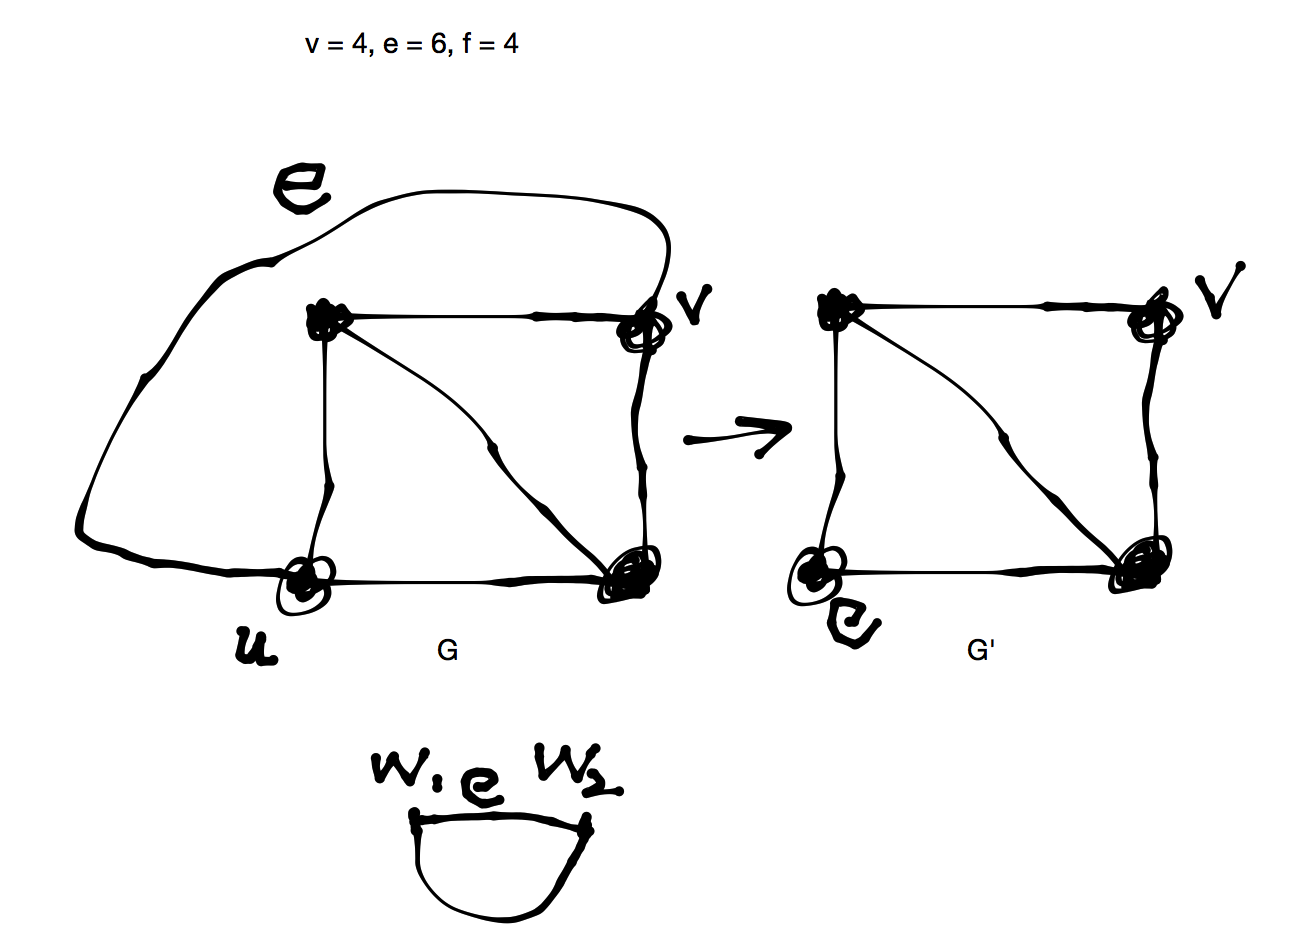
\includegraphics[width=\textwidth]{images/faces.png}

Verify $G'$ connected:

\begin{itemize}
	\item Given $u,v\in G',\ \exists$ path connecting $uv$. We know there exists such a path in $G$. If this path does not use $e$, it's still a path in $G'$. We are done.
	\item If our path uses $e$, we argue as follows:
	\begin{itemize}
		\item Because $e$ is on a cycle, $\exists$ a path in $G'$ from $w_1$ to $w_2$. So in $G'$, we have paths $u$ to $w_1$, $w_1$ to $w_2$, $w_2$ to $v$.
	\end{itemize}
\end{itemize}

The number of edges and faces both go down by one.

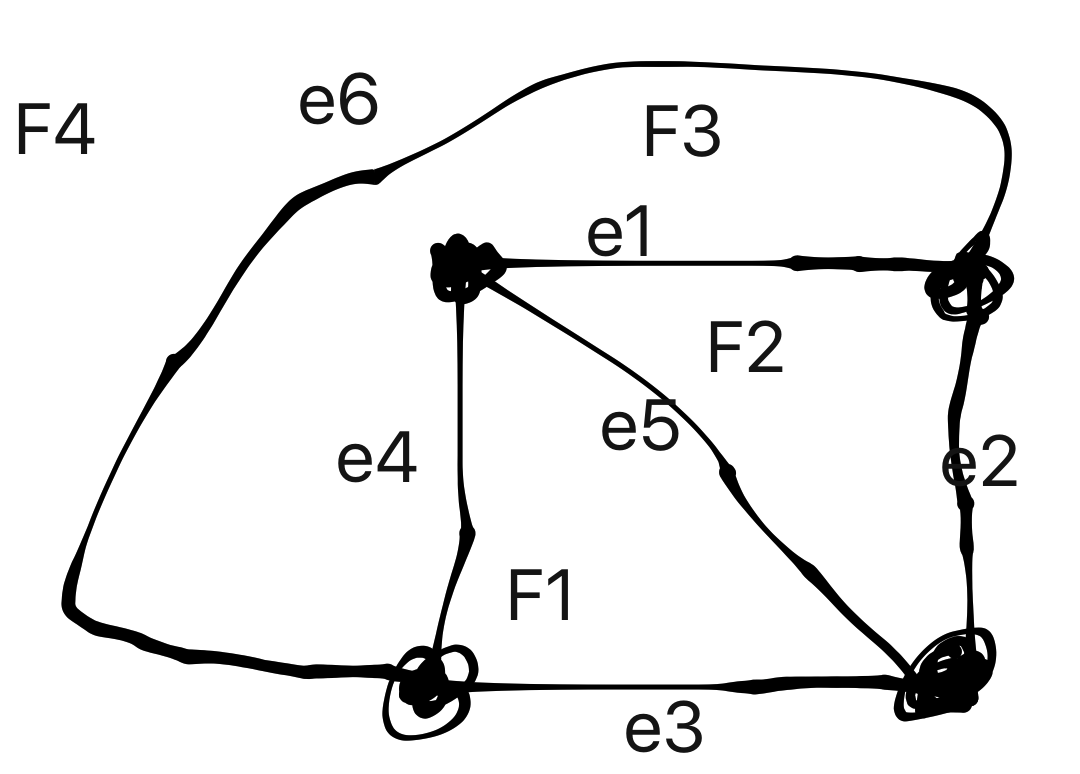
\includegraphics[width=\textwidth]{images/faces2}

$F_1:e_3, e_4, e_5$

$F_2:e_1, e_2, e_5$

$F_3:e_1, e_4, e_6$

$F_4:e_2, e_3, e_6$

\begin{itemize}
	\item Each edge appears twice.
	\item If simple, then each face has at least $3$ edges along its boundary.
\end{itemize}

\[3f\leq\sum^f_{i=1}\left(\text{the number of edges on boundary of the $i^{\text{th}}$ face}\right)= 2e\]

For a simple, planar graph: $3f\leq 2e$.

\paragraph{Corollary:} For a simple, connected, planar graph:

\[\begin{split}
	f&=2-v+e\\
	f&\leq \frac{2}{3}e\\
	\frac{2}{3}e&\geq f=2-v+e\\
	\frac{1}{3}e&\leq v-2\\
	e&\leq 3v-6
\end{split}
\]

For $K_5, v=5, e\leq 3\cdot 5-6=9, 4+3+2+1=10$. So $K_5$ is not planar.\\

For $K_{3,3}, v=6, e=9, 9\leq 3\cdot 6 - 6=12$. This does not suffice that $K_{3,3}$ is not planar.\\

If $G$ is a simple, planar graph with no 3-cycles then at least $4$ edges on boundary of any face.

\[4f\leq 2e\implies f\leq \frac12e\]

Therefore, for simple planar, connected graph, with no 3-cycles, \[\frac12e\geq f=2-v+e\implies\frac12e\leq v-2\implies e\leq 2v-4\]

So $K_{3,3}$ is not planar!
;
\paragraph{Kuratowski's Theorem:} A simple, connected graph $G$ is planar if and only if does not contain an expansion of $K_{3,3}$ or $K_5$ as a subgraph.

\paragraph{Conjecture:} Chromatic number of planar graphs should be less or equal to $4$.\\

Let's try to prove that every planar, simple graph has a vertex of small degree...

We know 

\[e\leq 3v-6\]

Note that \[\sum_{\text{vertices}}d(v_i)=2e\]

Multiple the above by $2$, $\sum_{\text{vertices}}d(v_i)=2e\leq 6v -12$

Sort of we ``proved'' that every planar, simple graph has a vertex of degree $\leq 5$...\\

\paragraph{Proposition:} Every simple, planar, connected graph $G$ has $\chi(G)\leq 6.$

\section{Friday's Lecture}

Continue yesterday's proof of proposition.

\paragraph{Proof:} Induction on the number of vertices.\\

Let $G$ be simple, planar, connected graph  with $n$ vertices.

Let $v$ be a vertex of degree $\leq 5$.

Consider $G'=G-\{v\}$.

If $G_1',\dots, G_k'$ are connected components of $G'$, each can be colored with $6$ colours by induction hypothesis.

Now since $v$ is adjacent to $\leq 5$ vertices, there are $\leq 5$ forbidden colours for $v$. Thus, we can extend a $6$-coloring of $G'$ to  a $6$-coloring of $G$.
\end{document}